\chapter{B1 board Schematics and Layout}

\begin{figure}
 \centering
 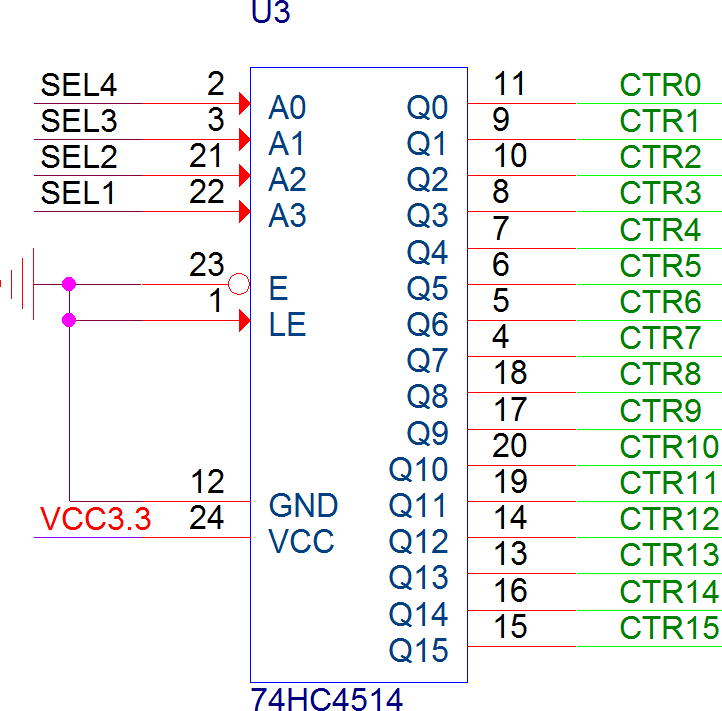
\includegraphics[width=0.9\textwidth]{B1_figures/b1_f1}
 \caption{I/O block of FPGA on the B2 schematic}
 \label{fig:b1_sch_1}
\end{figure}

\begin{figure}
 \centering
 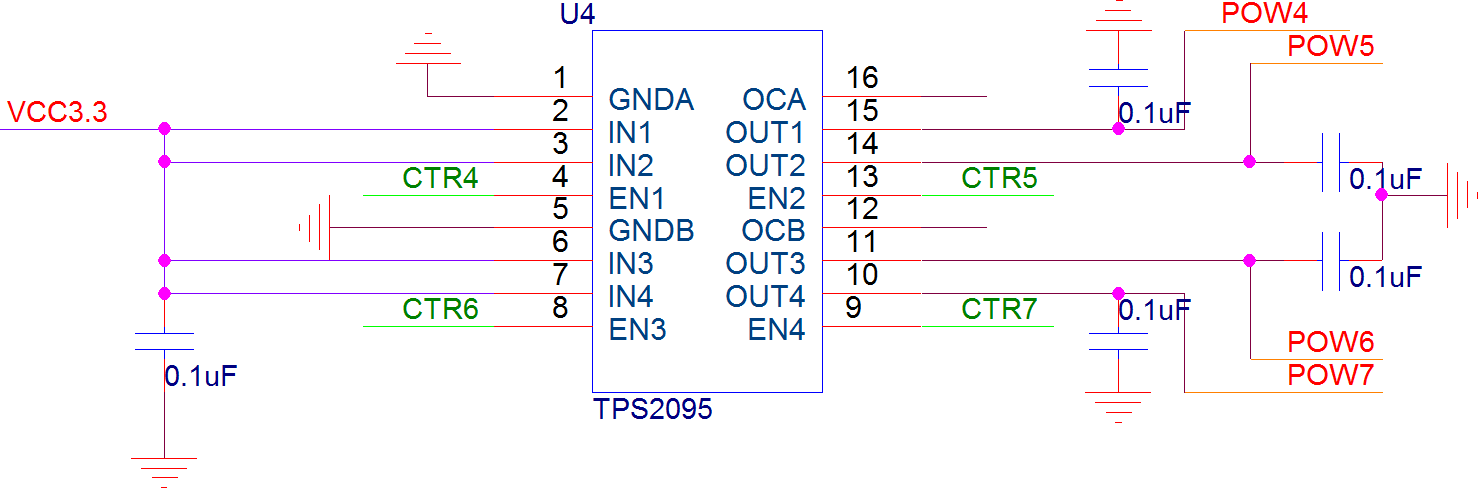
\includegraphics[width=0.9\textwidth]{B1_figures/b1_f2}
 \caption{Configuration block of FPGA on the B2 schematic}
 \label{fig:b1_sch_2}
\end{figure}

\begin{figure}
 \centering
 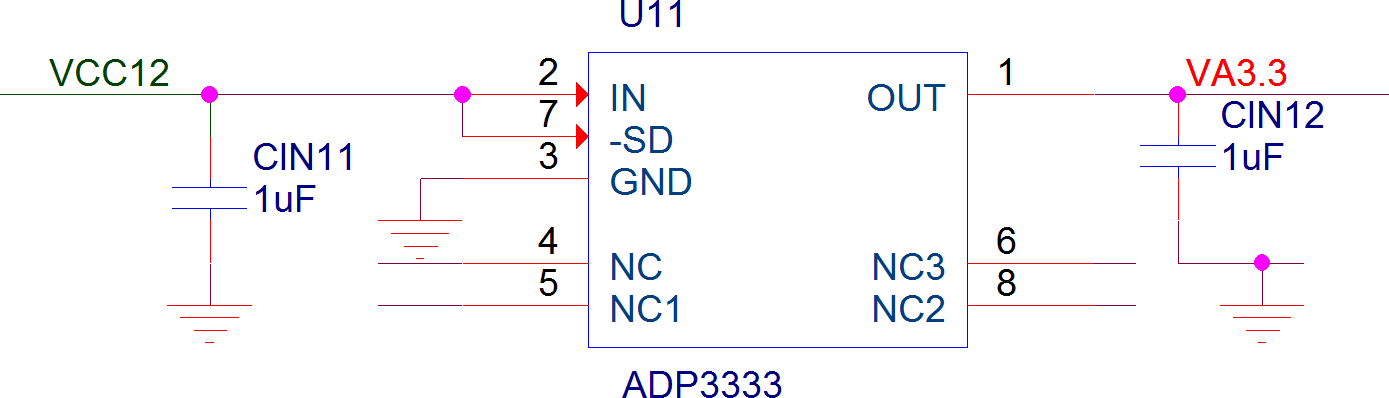
\includegraphics[width=0.9\textwidth]{B1_figures/b1_f3}
 \caption{Oscillator block on the B2 schematic}
 \label{fig:b1_sch_3}
\end{figure}

\begin{figure}
 \centering
 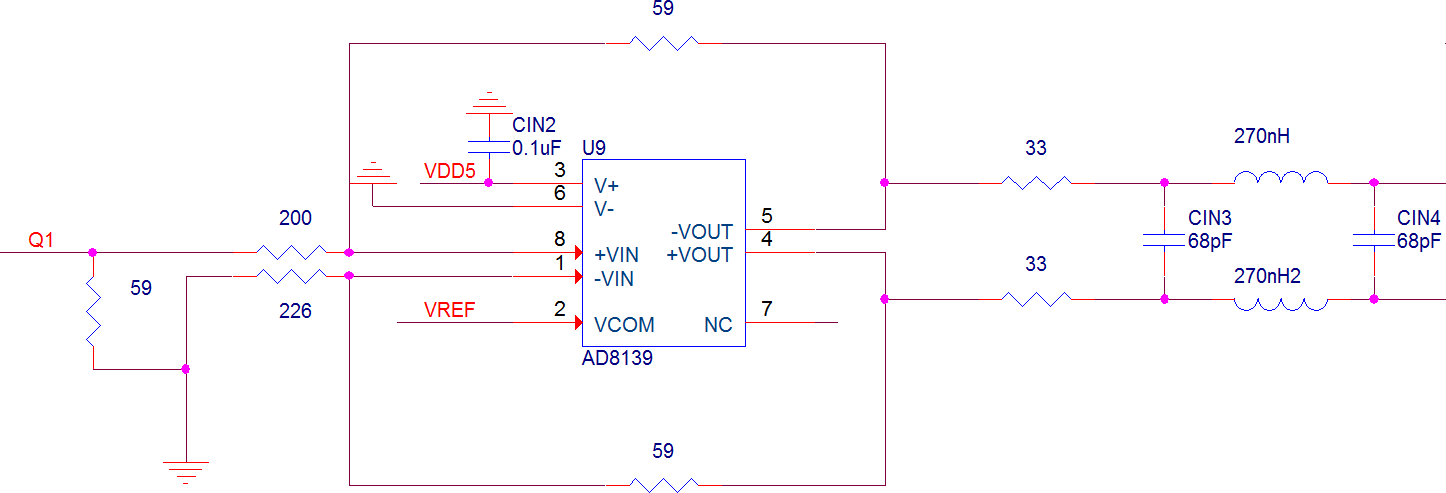
\includegraphics[width=0.9\textwidth]{B1_figures/b1_f4}
 \caption{Flash block on the B2 schematic}
 \label{fig:b1_sch_4}
\end{figure}

\begin{figure}
 \centering
 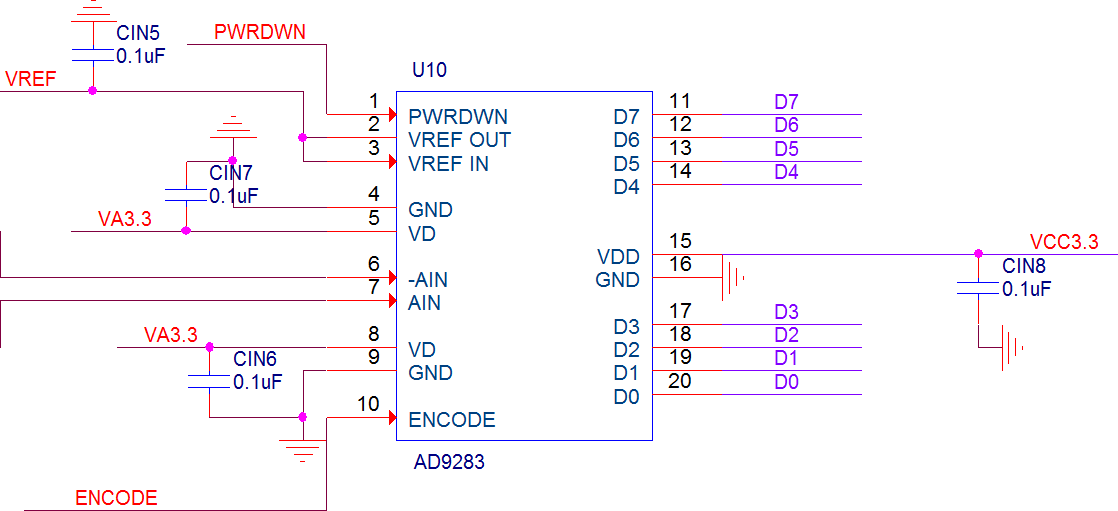
\includegraphics[width=0.9\textwidth]{B1_figures/b1_f5}
 \caption{Voltage regulator block on the B2 schematic}
 \label{fig:b1_sch_5}
\end{figure}

\begin{figure}
 \centering
 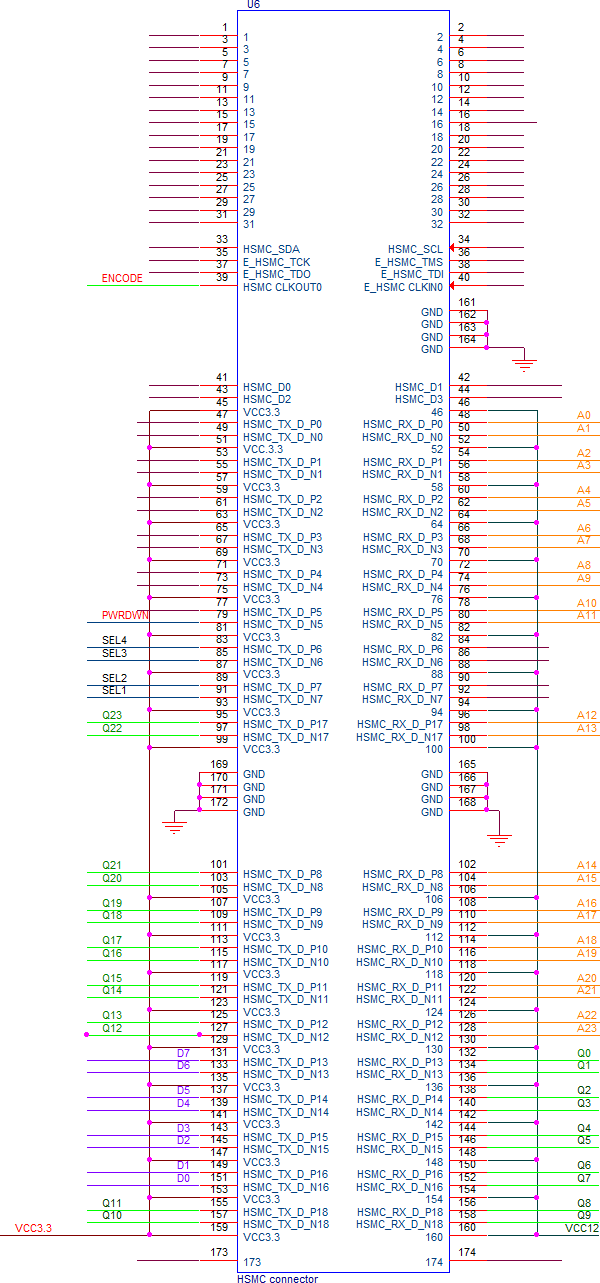
\includegraphics[width=0.7\textwidth]{B1_figures/b1_f6}
 \caption{Voltage regulator block on the B2 schematic}
 \label{fig:b1_sch_6}
\end{figure}